\chapter*{Цель работы}
Изучение архитектуры гетерогенных вычислительных систем и технологии разработки ускорителей вычислений на базе ПЛИС фирмы Xilinx.

В ходе лабораторной работы предлагается изучить основные сведения о платформе Xilinx Alveo U200, разработать RTL (Register Transfer Language, язык регистровых передач)) описание ускорителя вычислений по индивидуальному варианту, выполнить генерацию ядра ускорителя, выполнить синтез и сборку бинарного модуля ускорителя, разработать и отладить тестирующее программное обеспечение на серверной хост-платформе, провести тесты работы ускорителя вычислений.

\chapter*{Ход работы}

\section*{Функциональная схема разрабатываемой аппаратной системы}

На рисунке 1 представлена функциональная схема разрабатываемой аппаратной системы:
\FloatBarrier
\begin{figure}[h]
	\begin{center}
		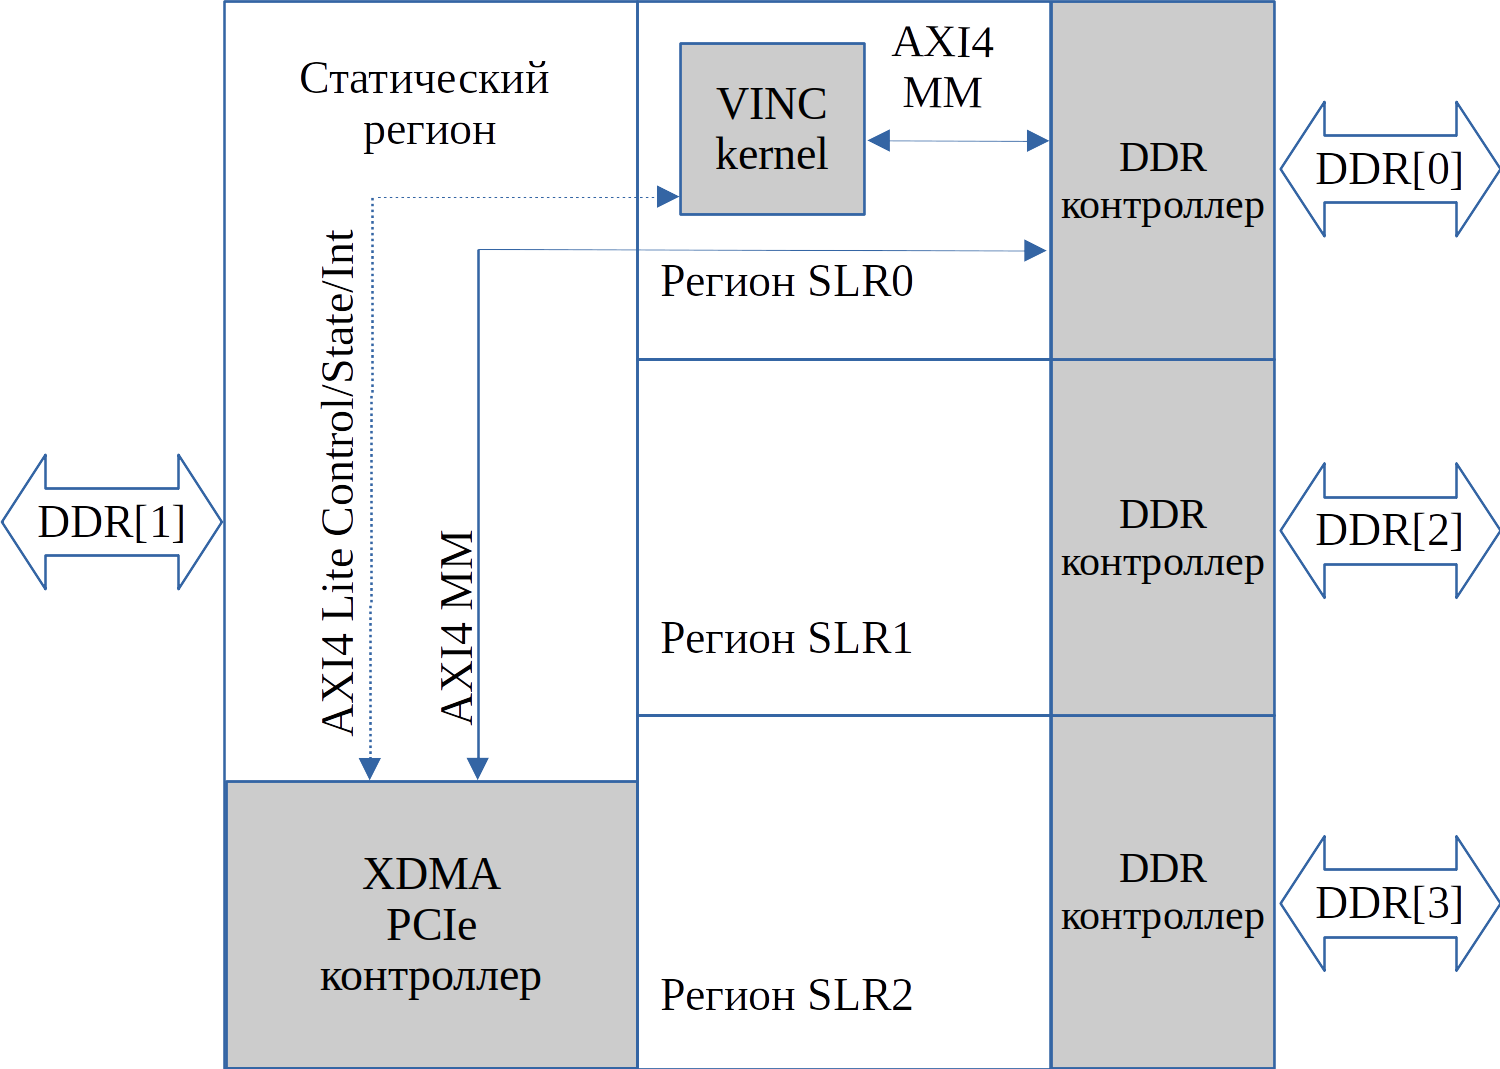
\includegraphics[width=\linewidth]{inc/schema.png}
	\end{center}
	\caption{Функциональная схема}
\end{figure}
\FloatBarrier

\section*{Копии экранов моделирования исходного проекта VINC}
В Vinc был создан проект под названием Alveo\_lab\_1.
Был запущен мастер RTL проекта VINC.
Summary получившегося результата представлено на рисунке 2.

\FloatBarrier
\begin{figure}[h]
	\begin{center}
		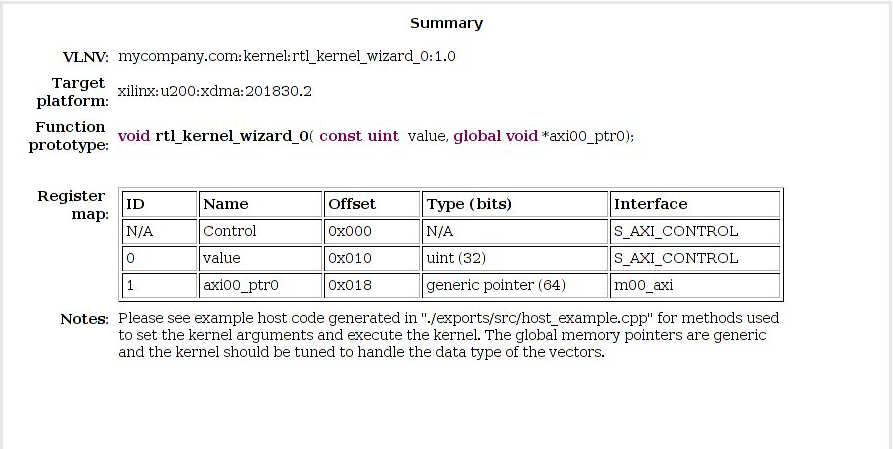
\includegraphics[width=\linewidth]{inc/summary.png}
	\end{center}
	\caption{Summary}
\end{figure}
\FloatBarrier

В результате был создан проект ядра ускорителя.
Каталог созданных файлов представлен на рисунке 3.

\FloatBarrier
\begin{figure}[h]
	\begin{center}
		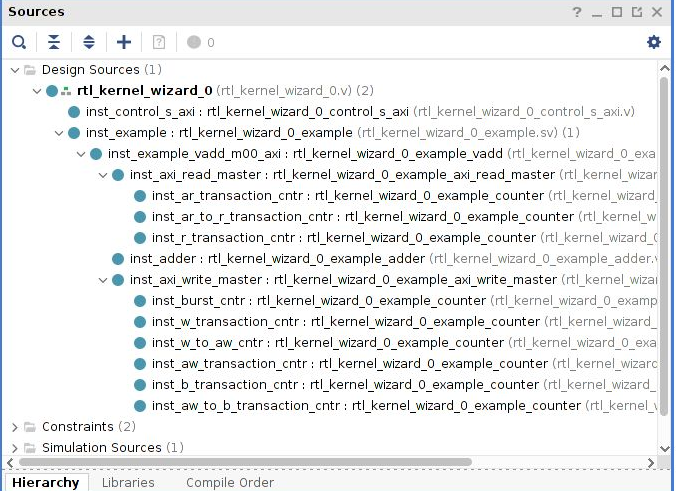
\includegraphics[]{inc/newfiles.png}
	\end{center}
	\caption{Каталог созданных файлов}
\end{figure}
\FloatBarrier

Последовательность событий транзакции чтения можно представить следующим образом: ARVALID→ ARREADY→ RVALID→ RREADY.

Последовательность событий транзакции записи: AWVALID→ AWREADY → WVALID → WREADY → BVALID → BREADY.

Была запущена и закончена симуляция проекта.
В результате была сформирована диаграмма, на которой можно отследить последовательности.

На рисунке 4 представлена одна транзакция чтения данных вектора на шине AXI4 MM из DDR памяти.

На рисунках 5 и 6 представлена одна транзакция записи результата инкремента данных на шине AXI4 MM. Так как сигналы не удалось уловить в один скриншот, транзакция разбита на две части.

На рисунке 7 представлена диаграмма инкремента данных в модуле.

\FloatBarrier
\begin{figure}[h]
	\begin{center}
		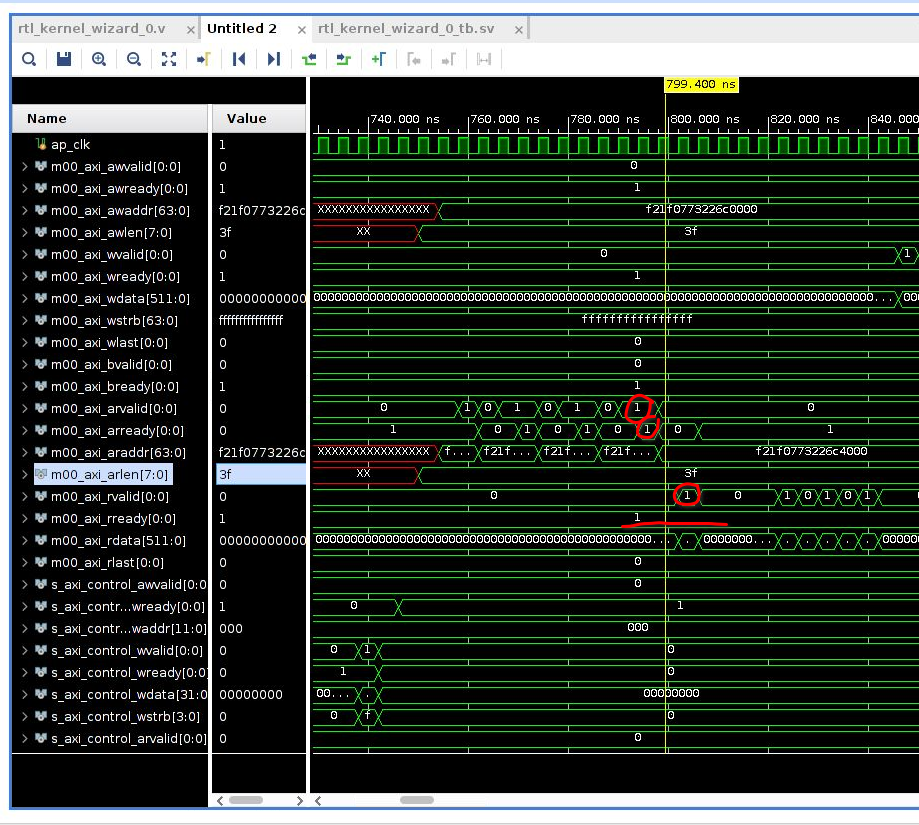
\includegraphics[width=\linewidth]{inc/read_original.png}
	\end{center}
	\caption{Транзакция чтения данных}
\end{figure}
\FloatBarrier

\FloatBarrier
\begin{figure}[h]
	\begin{center}
		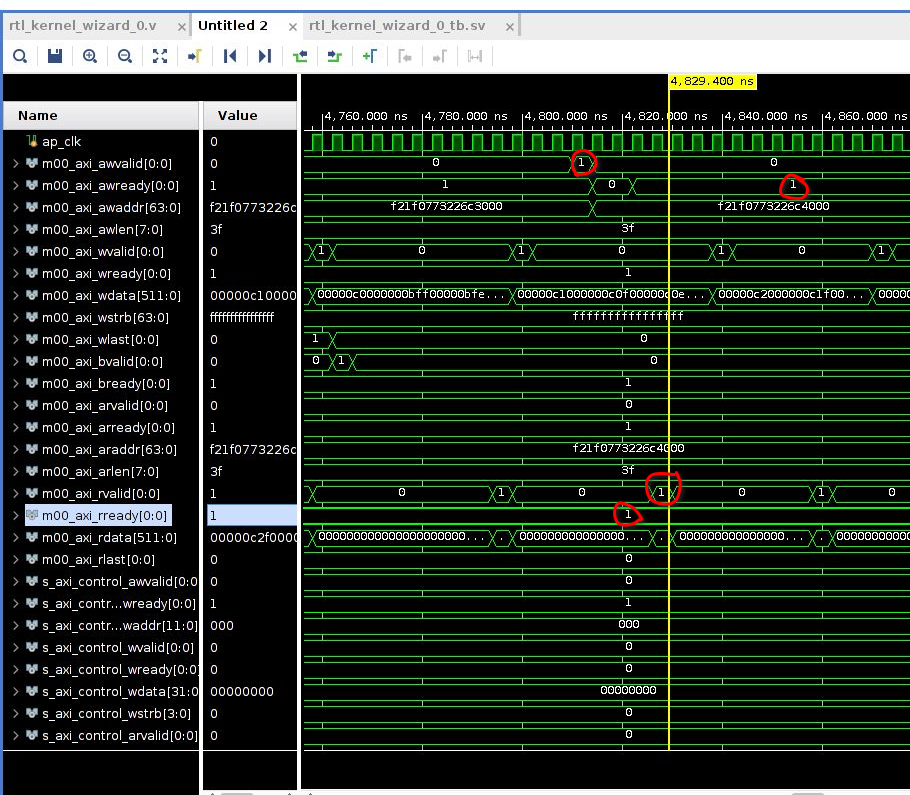
\includegraphics[width=\linewidth]{inc/write1_original.png}
	\end{center}
	\caption{Транзакция записи результата (часть 1)}
\end{figure}
\FloatBarrier

\FloatBarrier
\begin{figure}[h]
	\begin{center}
		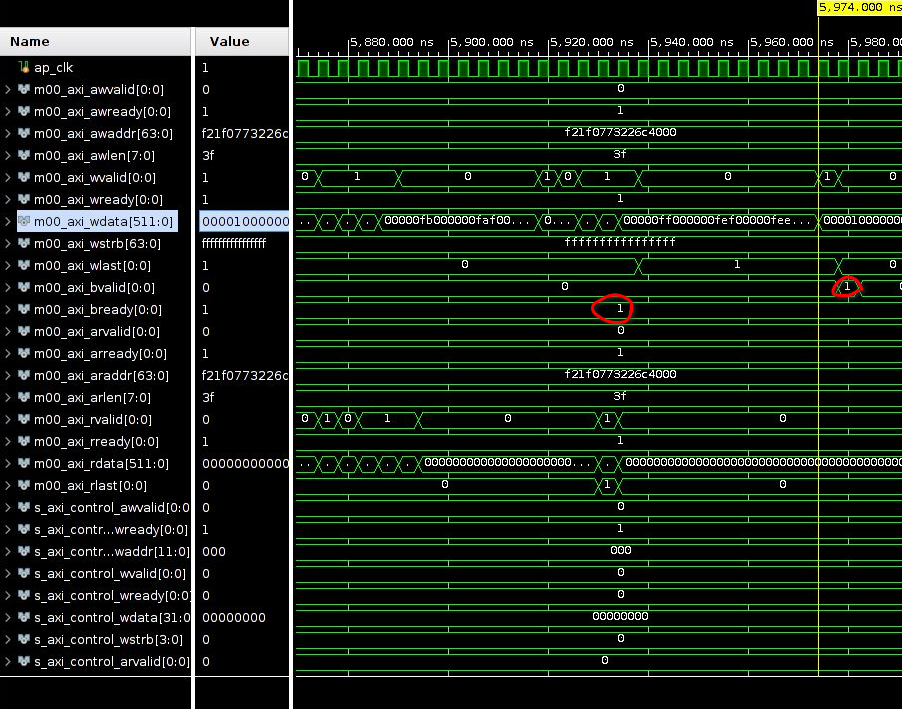
\includegraphics[width=\linewidth]{inc/write2_original.png}
	\end{center}
	\caption{Транзакция записи результата (часть 2)}
\end{figure}
\FloatBarrier

\FloatBarrier
\begin{figure}[h]
	\begin{center}
		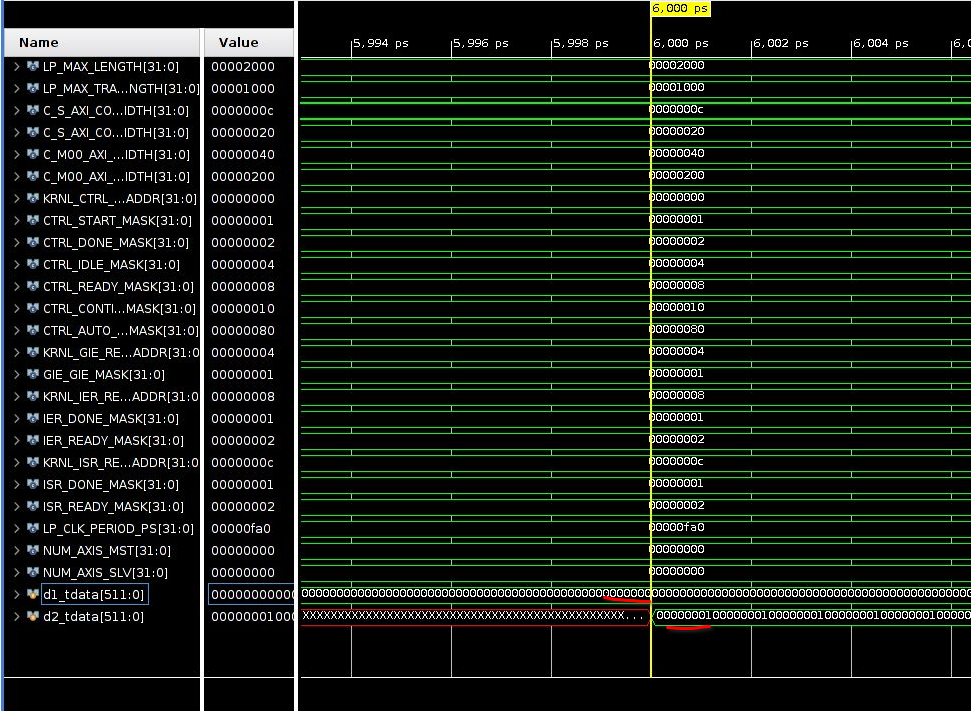
\includegraphics[width=\linewidth]{inc/inc_original.png}
	\end{center}
	\caption{Диаграмма инкремента данных}
\end{figure}
\FloatBarrier

\section*{Конфигурационный файл линковки}
Был сформирован *.xo файл, представляющий собой архив проекта Vivado с результатами синтеза.

Был создан конфигурационный файл alveo\_lab1.cfg.
Его содержимое представлено на листинге 1.
\begin{lstinputlisting}[caption=Конфигурационный файл линковки, 
basicstyle=\footnotesize\ttfamily, frame=single,breaklines=true]{src/conf.txt}
\end{lstinputlisting}

\section*{Содержимое файлов v++*.log и *.xclbin.info}
В системной консоли была запущена команда \textbf{screen}.
Была запущена линковка в сессии screen. Команда представлена на листинге 2.
\begin{lstinputlisting}[caption=Команда запуска линковки, 
	basicstyle=\footnotesize\ttfamily, frame=single,breaklines=true]{src/link.txt}
\end{lstinputlisting}

Вместе с генерацией файла *.xclbin был сгенерирован лог файл v++*.log и файл описания ресурсов *.xclbin.info.

На листинге 3 представлено содержимое лог файла *.log.

На листинге 4 представлено содержимое файла описания ресурсов *.xclbin.info.

\begin{lstinputlisting}[caption=Лог файл v++*.log, 
	basicstyle=\footnotesize\ttfamily, frame=single,breaklines=true]{src/log.txt}
\end{lstinputlisting}

\begin{lstinputlisting}[caption=Файл описания ресурсов *.xclbin.info, 
	basicstyle=\footnotesize\ttfamily, frame=single,breaklines=true]{src/info.txt}
\end{lstinputlisting}

\section*{Индивидуальное задание}
Мой вариант -- 6.
Функция по варианту:
\begin{equation}
R[i] = A[i] \& 0x76543210
\end{equation}

Регион по варианту: SLR1,DDR[1].

\section*{Измененный код *\_adder.v в соответствии с индивидуальным заданием}
В каталоге файлов в Vivago есть файл rtl\_kernel\_wizard\_0\_example.v. 

На листинге 5 представлена изменённая часть кода в соответствии с индивидуальным заданием.
Начальный код был закомментирован.

\begin{lstinputlisting}[caption=Изменённый код *adder.v, 
	basicstyle=\footnotesize\ttfamily, frame=single, breaklines=true]{src/code.txt}
\end{lstinputlisting}

\section*{Копии экранов модулирования измененного проекта VINC}
После этого было заново проведена сборка ядра и моделирование.

На рисунке 8 представлена одна транзакция чтения данных вектора на шине AXI4 MM из DDR памяти.

На рисунках 9 и 10 представлена одна транзакция записи результата инкремента данных на шине AXI4 MM. Так как сигналы не удалось уловить в один скриншот, транзакция разбита на две части.

На рисунке 11 представлена диаграмма инкремента данных в модуле.

\FloatBarrier
\begin{figure}[h]
	\begin{center}
		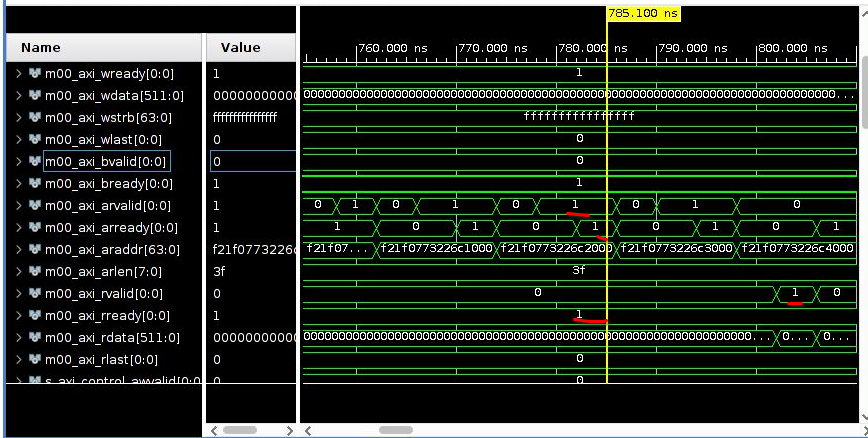
\includegraphics[width=\linewidth]{inc/read_my.png}
	\end{center}
	\caption{Транзакция чтения данных (после моделирования изменённого проекта)}
\end{figure}
\FloatBarrier

\FloatBarrier
\begin{figure}[h]
	\begin{center}
		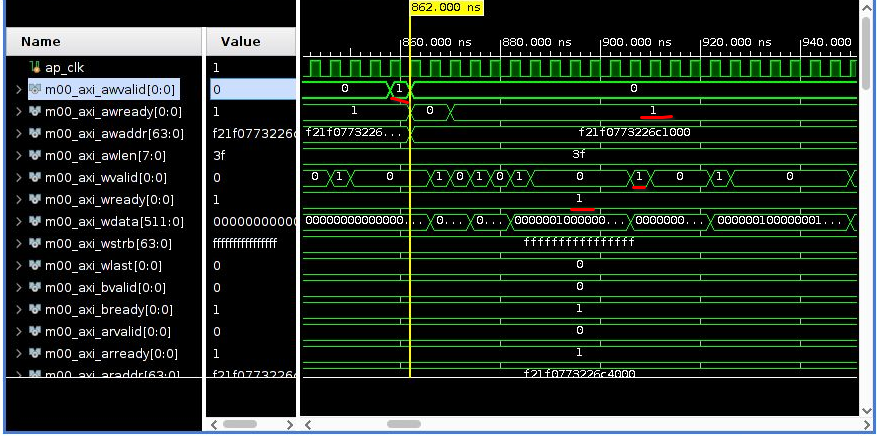
\includegraphics[width=\linewidth]{inc/write_my_1.png}
	\end{center}
	\caption{Транзакция записи результата (часть 1) (после моделирования изменённого проекта)}
\end{figure}
\FloatBarrier

\FloatBarrier
\begin{figure}[h]
	\begin{center}
		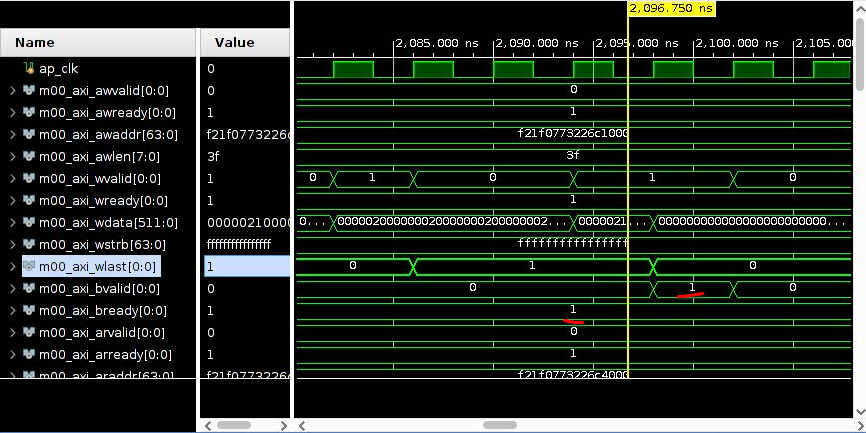
\includegraphics[width=\linewidth]{inc/write_my_2.png}
	\end{center}
	\caption{Транзакция записи результата (часть 2) (после моделирования изменённого проекта)}
\end{figure}
\FloatBarrier

\FloatBarrier
\begin{figure}[h]
	\begin{center}
		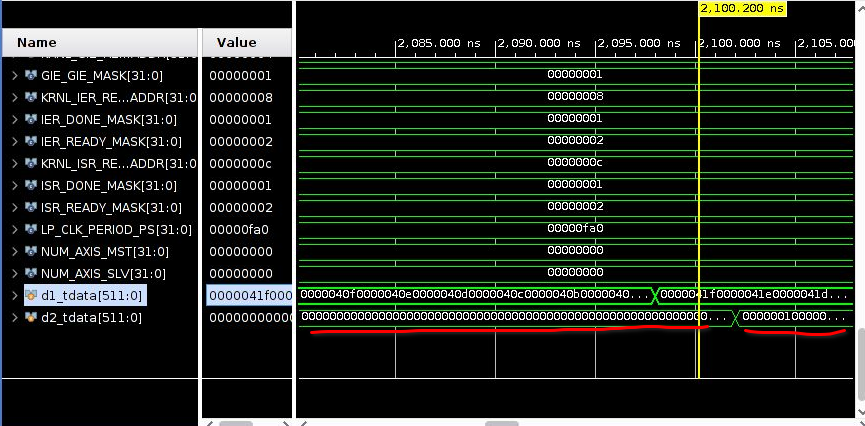
\includegraphics[width=\linewidth]{inc/inc_my.png}
	\end{center}
	\caption{Диаграмма инкремента данных}
\end{figure}
\FloatBarrier

При этом в соответствии с индивидуальным вариантом был изменён файл проверки rtl\_kernel\_wizard\_0\_control\_s\_axi.v

На листинге 6 приведена изменённая часть кода файла проверки:
\begin{lstinputlisting}[caption=Изменённый код *adder.v, 
	basicstyle=\footnotesize\ttfamily, frame=single,breaklines=true]{src/new_check.txt}
\end{lstinputlisting}

Успешный результат тестирования представлен на рисунке 12.

\FloatBarrier
\begin{figure}[h]
	\begin{center}
		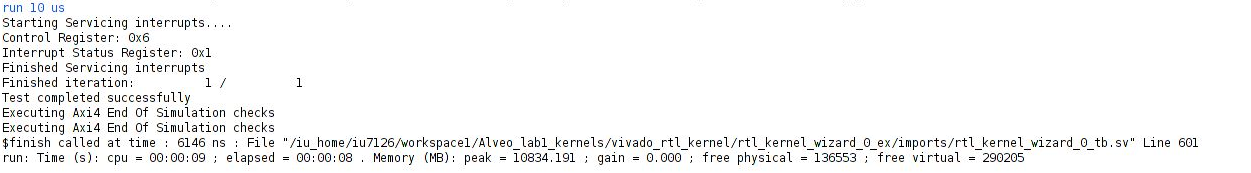
\includegraphics[width=\linewidth]{inc/test_completed.png}
	\end{center}
	\caption{Результат тестирования}
\end{figure}
\FloatBarrier

\section*{Код модифицированного модуля}
Была выполнена линковка, аргументы такие же, как и при первой итерации.

Также был изменён код модуля host\_example.cpp.

На листинге 7 представлена часть кода модуля, которая была изменена.
\begin{lstinputlisting}[language=C++, caption=Изменённый код модуля host\_example.cpp, 
	basicstyle=\footnotesize\ttfamily, frame=single,breaklines=true]{src/host.cpp}
\end{lstinputlisting}

\section*{Результаты запуска}
На рисунке 13 представлен скрин успешного запуска:

\FloatBarrier
\begin{figure}[h]
	\begin{center}
		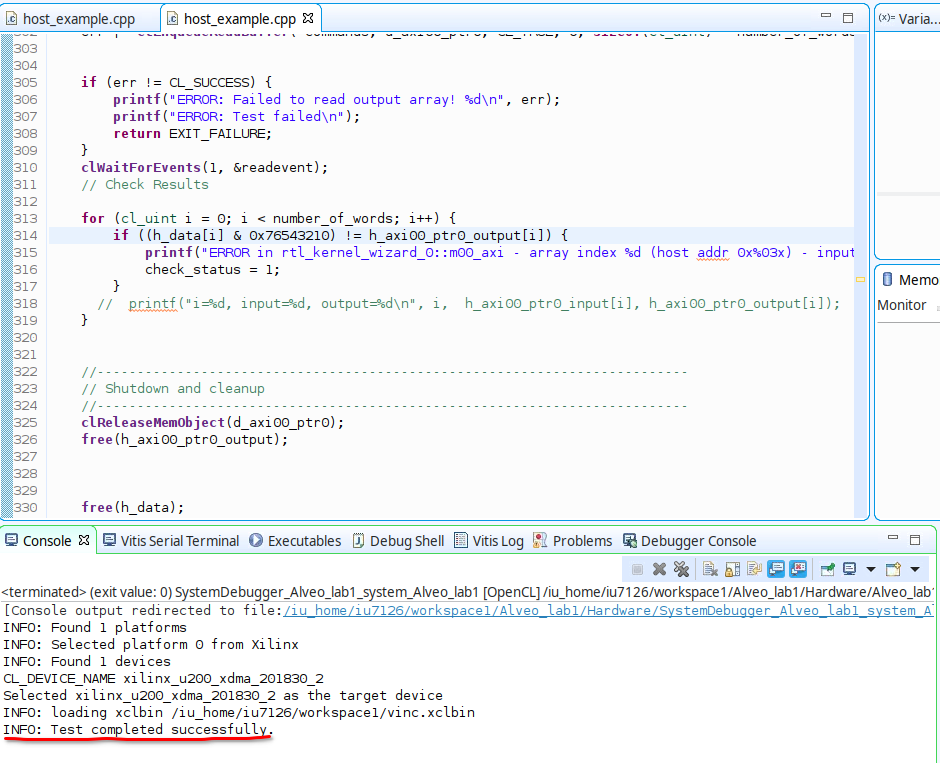
\includegraphics[width=\linewidth]{inc/final_result.png}
	\end{center}
	\caption{Результат тестирования}
\end{figure}
\FloatBarrier

\section*{Контрольные вопросы}

\subsection*{1. Назовите преимущества и недостатки XDMA и QDMA платформ}
У QDMA есть следующие преимущества:
\begin{itemize}
	\item позволяет передавать поток данных непосредственно в логику FPGA параллельно с их обработкой.
	\item предоставляет разработчикам прямое потоковое соединение с низкой задержкой между хостом и ядрами.
	\item включает высокопроизводительный DMA, который использует несколько очередей, оптимизированных как для передачи данных с высокой пропускной способностью, так и для передачи данных с большим количеством пакетов.
\end{itemize}

\subsubsection*{2. Назовите последовательность действий, необходимых для инициализации ускорителя со стороны хост-системы.}

\begin{enumerate}
	\item Хост получает все платформы.
	\item Хост выбирает имя платформы Xilinx.
	\item Хост получает Id устройства.
	\item Хост получает информацию об устройстве.
	\item Создается контекст для переменных.
	\item Создается команда для устройста-ускорителя.
\end{enumerate}

\subsubsection*{3. Какова процедура запуска задания на исполнения в ускорительном ядре VINC.}

\begin{enumerate}
	\item Данные из .xclbin копируются из ОЗУ в локальную память ускорителя посредством DMA.
	\item В памяти устройства-ускорителя создается исполняемый файл.
	\item Те данные, которые подлежат обработке, копируются из ОЗУ в локальную память усокрителя посредством DMA.
	\item Указываются необходимые параметры и запускается программа на ускорителе.
	\item В конце выполняется чтение готовых данных. 
\end{enumerate}

\subsubsection*{4. Опишите процесс линковки на основании содержимого файла v++\_*.log.}

\begin{enumerate}
	\item Анализ профиля устройства. Анализ конфигурационного файла. Поиск необходимых интерфейсов.
	\item FPGA linking synthesized kernels to platform
	\item FPGA logic optimization (оптимизация логики ПЛИС) для минимизации задержки.
	\item FPGA logic placement (размещение логики ПЛИС, то есть выбор конкретного мета для определенного логического блока). 
	\item FPGA routing (маршрутизация ПЛИС)
	\item FPGA bitstream generation (генерация битового потока ПЛИС, то есть генерация файла  [*.xclbin]).
\end{enumerate}